Since we're past the one year point in this blog it is interesting to
look back at what was being talked about one year ago. On this day last
year I wrote:

\begin{quote}
\begin{figure}
\centering
\pandocbounded{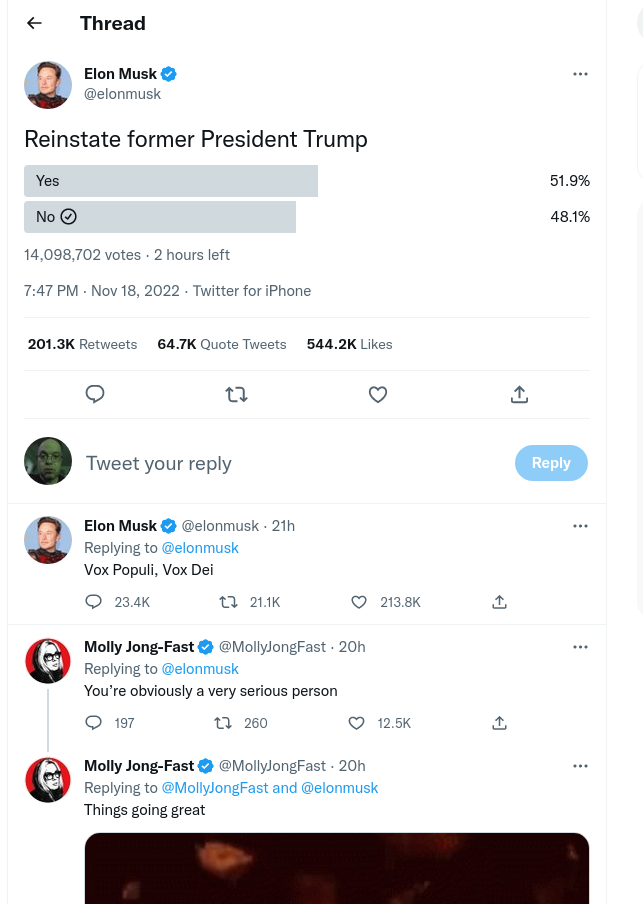
\includegraphics[keepaspectratio]{\%7B\%7Bsite.url\%7D\%7D/img/MuskCrazyIdea.png}}
\caption{Clipped screenshot of a poll on Twitter run by Elon Musk
concerning reinstating Donald John Trump to the platform}
\end{figure}

\emph{Well, that's frankly rather disturbing. Mr.~Musk really wants to
appeal to a core audience of craziness. Keeping the Trump dream alive
definitely resonates with part of the economy, perhaps. It is part of
the economy I truly do not want to take part in. The former president
has done so many wild things that the Justice Department brought in a
former war crimes prosecutor who handled cases }from Kosovo* to handle
the January 6th and classified documents investigations. Wouldn't a
reasonable person think that perhaps that's a clue that we may be
dealing with a supervillain here?*

\emph{That screenshot was from the middle of the afternoon on Saturday.
Later on Saturday this popped up on my Apple Watch:}

\begin{figure}
\centering
\pandocbounded{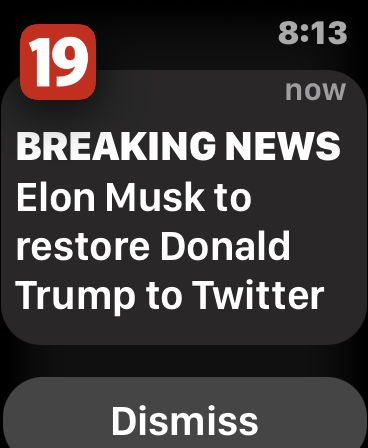
\includegraphics[keepaspectratio]{\%7B\%7Bsite.url\%7D\%7D/img/trump-restored-twitter.png}}
\caption{Screenshot from watchOS of a notification from the Cleveland19
app indicating that Donald Trump is seeing his ban from Twitter being
rescinded}
\end{figure}

\emph{We're seeing bad things happen now!}
\end{quote}

One year later we've found that Mr.~Trump is sticking with Truth Social
and isn't really touching his restored X/Twitter account. He's becoming
increasingly kooky in what he is posting. X/Twitter is increasingly
becoming a cesspool and advertisers are bailing out again after Elon
Musk supported some vile anti-semitic content.

Things haven't gotten better as time has gone by.
